

\section{Discussions}

\subsection{Countermeasure}

The success of our attack depends on three factors: (1)
knowledge of the pattern grid; (2) a decent
quality video footage allowing the algorithm to track the fingertip movement;
(3) successfully identifying a video segment that captures the entire process of pattern drawing.

For the first factor, the attacker can obtain the relevant information by simply looking the pattern grid
of the target operating system or application.
Randomization techniques such as
randomized pictures~\cite{biddle2012graphical,hossein2015fortifying}, which randomly shuffle the location
of touch points each time, could be a solution.
However, randomization-based solutions often come at the cost of poorer
usability. This can prevent them to be used at a large scale.
Regarding the second factor, there are ways, such as
KALEIDO~\cite{zhang2015kaleido}, to prevent unauthorized videotaping by
dynamically changing the colour and brightness of the screen to confuse the
filming camera. A non-technical solution for this aspect would be to educate users to
fully cover their fingers when drawing a pattern. But doing this on a large-screen device could be awkward especially when the device is held by one hand.



For the third factor, the attacker's solution depends on the type of the
pattern. For a screen lock, pattern drawing is the first activity (except for
receiving a phone call or making an emergency call) when the device is
retrieved. Therefore, identifying the video segment is straightforward. When
the pattern is used by applications, we have observed that users typically
pause for a few seconds before or after entering the pattern. Therefore, an
experienced attacker should also be able to identify the video segment in
case our automatic algorithm (presented in Section~\ref{sec:identify}) fails
to do so. A potential countermeasure is to mix pattern unlocking with other
on-screen activities. For examples, before and after pattern drawing, the
system can ask the user to type in a sentence using a Swype-like method or to
draw some graphical shapes. The problem of this approach is it may annoy
users by asking them to do more, especially for screen unlocking -- an
activity that is performed
many times a day.

%De Luca \emph{et. al} proposed a new touch screen authentication using both the pattern and the touch screen data(pressure, time, speed, etc.)~\cite{de2012touch}, However, this design decreases the usability of

\begin{figure}[!t]
        \centering
        \subfigure{
             \begin{minipage}[t]{0.13\textwidth}
                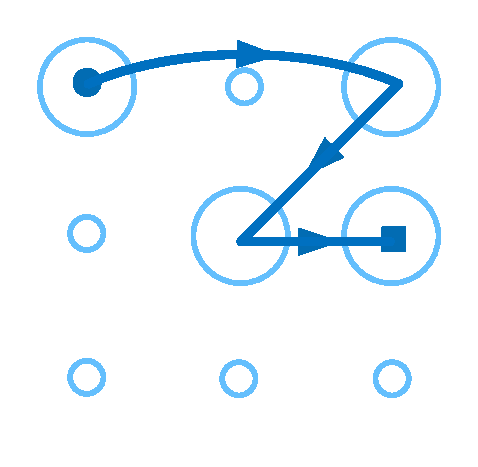
\includegraphics[width=\textwidth]{fig/protection1.pdf}\\
                \centering \footnotesize (a)
             \end{minipage}
        }
        \hspace{0.1cm}
        \subfigure{
             \begin{minipage}[t]{0.13\textwidth}
                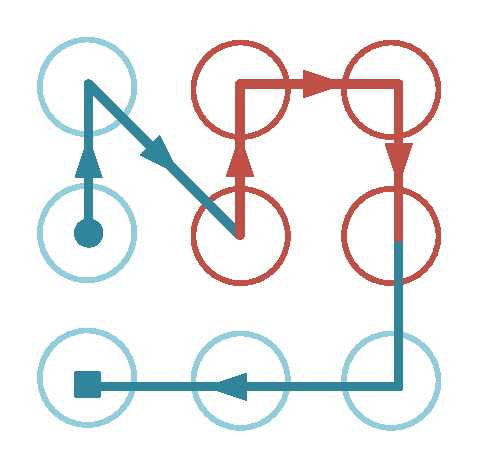
\includegraphics[width=\textwidth]{fig/protection2.pdf}\\
                \centering \footnotesize (b)
             \end{minipage}
        }
        \hspace{0.1cm}
        \subfigure{
             \begin{minipage}[t]{0.13\textwidth}
                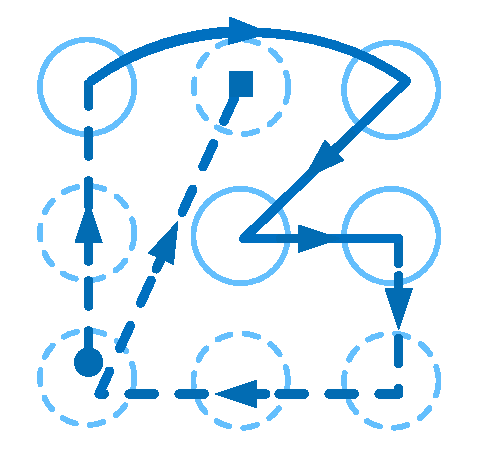
\includegraphics[width=\textwidth]{fig/protection3.pdf}\\
                \centering \footnotesize (c)
             \end{minipage}
        }
        %\hspace{0.2cm}
        \subfigure{
             \begin{minipage}[t]{0.145\textwidth}
                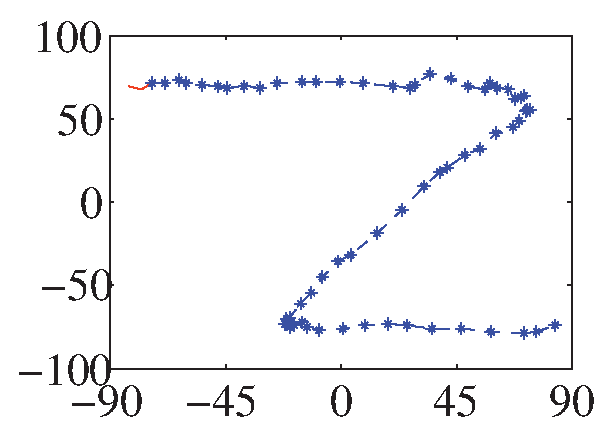
\includegraphics[width=\textwidth]{fig/protection1-1.eps}\\
                \centering \footnotesize (d)
             \end{minipage}
        }
        \hspace{-0.3cm}
        \subfigure{
             \begin{minipage}[t]{0.15\textwidth}
                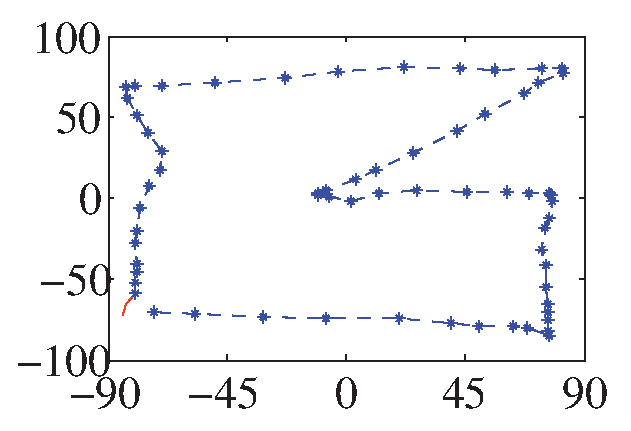
\includegraphics[width=\textwidth]{fig/protection2-1.eps}\\
                \centering \footnotesize (e)
             \end{minipage}
        }
        \hspace{-0.3cm}
        \subfigure{
             \begin{minipage}[t]{0.15\textwidth}
                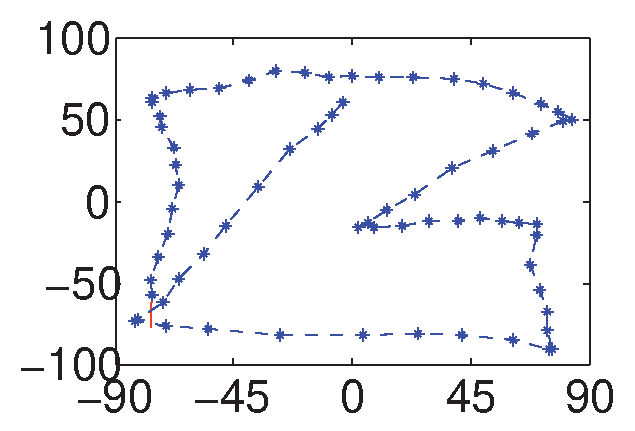
\includegraphics[width=\textwidth]{fig/protection3-1.eps}\\
                \centering \footnotesize (f)
             \end{minipage}
        }
        \caption{Examples of our new pattern lock mechanism. A true pattern of solid lines is shown
        in (a). We propose to make two changes to form a pattern.
        Our first change allows the user to skip some dots when creating a pattern.
        For example, in (a) the central dot in the first line is skipped.
        Our second change requires the user to draw a given random pattern structure (e.g. the dash lines in b and c)  before or after drawing the true pattern.
        The tracked fingertip trajectories of a, b, and c are shown in d, e, f respectively.
        The first change makes it difficult for the tracking algorithm to identify which dots are skipped, and the second change
         forces the attacker to use multiple video recordings to identify the true pattern. As a result, this new pattern lock mechanism decreases the
        effectiveness of the video-based attack.
        }
        \label{fig:protection}
    \end{figure}

\subsection{A Possible Remedy}
\label{section: potential-remedy}
We propose a countermeasure to make it difficult to obtain a meaningful video footage. When design the approach, we try
to find a balance between the usability and the security. Our approach requires making two  changes to the pattern
lock: (1) when forming a pattern the user can skip some of the dots in a vertical, horizontal, or diagonal line
(e.g. the central dot of the top line is skipped in Figure~\ref{fig:protection} a); (2) before or after drawing the correct pattern, the user is asked to draw a given random
pattern to confuse the attacker (e.g. sub-figures b and c in Figure~\ref{fig:protection}). For the second change, we relax the rules for
creating a pattern to allow a touching dot to be visited multiple times (e.g. the bottom-left dot at
Figure~\ref{fig:protection} c is visited twice). Further, for purpose of increasing the number of candidate
patterns, we also change the rule that a previously unvisited dot can be bypassed if it is part of a horizontal,
vertical or diagonal line segment of the pattern.

The two changes mentioned above can significantly decrease the effectiveness of the attack.
Our first change allows the user to skip some dots, which makes it difficult for the tracking algorithm to identify which dots
are skipped (because the video-camera is not able to precisely capture depth information). The
second change makes it harder for the attacker to identify which part of the track pattern is the true pattern.
Figures~\ref{fig:protection} d, e, and f respectively show the tracked fingertip trajectory of the
patterns shown in Figures~\ref{fig:protection} a, b, and c. The tracked trajectories have been
transformed to the user's perspective for presentation. As can be seen from the tracked trajectories,
using a pattern that is directly mapped from the trajectory will lead to a failed attempt. Because each time
the system will ask the user to draw a random pattern structure, directly use the tracked pattern (ignore
the skipping dots) will not be accepted by the system.


To understand how these changes affect the user experience, we specifically asked our participants if they feel these rules decrease
the usability. The answers from the all 10 participants are negative (i.e., they do not think this method decrease the usability).
We believe our countermeasure makes it harder to launch the attack as the adversary will now need to
identify which part of the drawing is the true pattern.
To prove hypothesis, we applied our attacking method to reconstruct 30 patterns generated by this new pattern lock design.
Our experiments show that only two out of the 30 patterns can be cracked by our attacking method.
After having a close look of the two successful cracked patterns, we found that they have little difference with the true patterns.
This experiment confirms that the introduction of randomness can improve the pattern lock security under video-side channel attacks.

It is worth mentioning that our countermeasure is not a panacea. In fact, finding a balance between the
usability and security for graphical passwords remains an open problem~\cite{Abdullah2008Towards}.
Even with our countermeasure, an attacker can still use multiple videos that record the same user when doing pattern
drawing to find the common pattern structure (which will likely to be the true pattern). Therefore, while our
countermeasure is simple to implement and can increase the overhead for performing the attack, an experienced
adversary could still successfully launch the attack.


%Moreover, comparing to original system, this can frustrate shoulder-surfing attack as well as video-based attack as the attacker cannot recognize the correct pattern in spite of see or reconstruct the pattern. Furthermore, this improved scheme precede biometric-based scheme such as face recognition~\cite{turk1991face} and iris recognition~\cite{sanchez2001iris} in terms of revocability.


\subsection{Implications}
While pattern lock is preferable by many users~\cite{androidstudy}, this     work shows
that it is vulnerable under video-based attacks. Our attack
is able to break most patterns in five attempts. Considering Android
allows five failed attempts before automatically locking the device, our work
shows that this default threshold is unsafe. We demonstrated that, in contrast to many users'
perception, complex patterns actually do not provide stronger protection over simple patterns under our attack.

It is worth mentioning that our approach is only one of the many attacking
methods that researchers have demonstrated. Examples of these attacks include
video-based attacks on keystroke-based authentication~\cite{shukla2014beware,yue2014blind}, sensor-based attacks for
pattern lock~\cite{zhang2016privacy}. Authentication methods that combine different
authentication methods~\cite{de2012touch,stefan2012robustness,lingsecure,mannan2007using} to constantly check the user's identity could be
a solution. %However, due to stealthiness and diversity of
%such attacks, there may not exist an ``one-size-fits-all" solution.



   % \FIXED{In this section, we discuss some possible defense strategies against video-based attacks proposed in this paper. For other attack approaches introduced in related work, there are some other defense strategies. In order to protect the text-based passwords, randomized keyboard \cite{hoanca2005screen,shin2010device,kim2012keypad}have been proposed against computer vision based attacks.}
%
%    \FIXED{Indeed, there are also some other authentication approaches immune to video-based attack. With the widely use of various diversity of sensors embed into smartphones, Shahzad \cite{shahzad2013secure} propose a protection approach by multiple information collected by sensor such as gyroscope and accelerator. This defense approach, unfortunately, seems to be attacked by Serwadda \cite{serwadda2013kids}, who proposed a new attack method for multi-authenticated information produced by sensors. In addition, biometric-rich locking mechanisms have been proposed \cite{kalal2012tracking,hoanca2005screen}. The successful use of fingerprint authentication on iPhone is a positive example for preventing the video-based attack. But recently researcher points that fingerprint can be forged~\cite{shin2009dictionary}, making the fingerprint authentication mechanism is also unsafe.}
%
%    \FIXED{To prevent the video from filming secretly, Lan Z proposes the KALEIDO~\cite{zhang2015kaleido}, a system that prevents unauthorized users from recording a high-quality redisplay on a screen by taking full use of light difference between the screen-eye channel and the screen-camera channel. Thus, in our further work, based on such limited disparities, we can design a system that prevent the attacker from implementing video-based attacks. Specifically, to obstruct the video filming, the certain frequency of light can be launched by touch-screen during drawing the pattern lock.}
%
%    \FIXED{With the advent of new technologies, however, there are still some novel attack methods arouse. Due to stealthiness and diversity of such attacks. There are not a uniform countermeasure to protect our private data from leakage. The best approach for protecting privacy is enhance safety consciousness and if possible, do not input your private information in public places.}
